% ===================== Who&When =====================
\subsection{Who\&When}\label{ds:who_and_when}
\badgerow{\naturalbadge\ \okbadge\ \lbl{agent + step}\ \lbl{MAS}\ \lbl{GAIA / AssistantBench}}

\begin{identity}
Paper & \emph{Which Agent Causes Task Failures and When? On Automated Failure Attribution of LLM Multi-Agent Systems} --- Zhang et al., ICML 2025 (spotlight), arXiv:2505.00212 \cite{zhang2025who}\\
Links & \href{https://huggingface.co/datasets/Kevin355/Who_and_When}{HF \code{Kevin355/Who\_and\_When}} \textperiodcentered\ \href{https://github.com/mingyin1/Agents_Failure_Attribution}{GitHub \code{mingyin1/Agents\_Failure\_Attribution}}\\
License & none stated on the dataset card or repo (paper CC BY 4.0); underlying queries from GAIA and AssistantBench\\
Status & downloaded in full, ungated; 9.5 MB; \code{data/who\_and\_when/} (184 JSON logs + 2 parquet files)\\
\end{identity}

\paragraph{Description} Who\&When is the benchmark that defined the task (\S\ref{sec:intro}): every record is the output log of a multi-agent run that \emph{failed} a GAIA or AssistantBench query, plus three labels---\code{mistake\_agent} (who), \code{mistake\_step} (when: a 0-based index into \code{history}) and a free-text \code{mistake\_reason}. Failures are natural (no injection). Two subsets come from two very different MAS:
\begin{itemize}
\item \textbf{Algorithm-Generated} (126 logs): teams assembled automatically per task by \emph{CaptainAgent} (AG2, GPT-4o)---a handful of \code{*\_Expert} agents plus a \code{Computer\_terminal}. 82 distinct expert names appear as blamed agents.
\item \textbf{Hand-Crafted} (58 logs): \emph{Magentic-One} (Orchestrator, WebSurfer, FileSurfer, Coder/Assistant, ComputerTerminal) on 28 AssistantBench and 30 GAIA tasks.
\end{itemize}
In total 184 logs from 127 distinct MAS configurations. \textbf{Annotation}: three experts, three rounds (independent labelling with uncertainty flags on 15--30\% of cases, consensus discussion, cross-validation); 23--31 h per annotator; no agreement coefficient reported. The decisive step is defined as the earliest step whose correction would have made the run succeed---a single-root-cause assumption later questioned by MP-Bench.

\paragraph{Metrics and baselines} Agent-level and step-level exact-match accuracy, with or without the ground-truth answer given to the attributor. Three prompting strategies were compared (GPT-4o, with ground truth; agent\,/\,step accuracy in \%):

\begin{center}\small
\begin{tabular}{@{}lcc@{}}\toprule
Method & Alg.-Generated & Hand-Crafted\\\midrule
Random & 29.1 / 19.1 & 12.0 / 4.2\\
All-at-Once & \textbf{54.3} / 12.5 & \textbf{55.2} / 5.3\\
Step-by-Step & 35.2 / \textbf{25.5} & 34.5 / 7.0\\
Binary Search & 44.1 / 24.0 & 51.7 / 6.9\\\bottomrule
\end{tabular}
\end{center}
Reasoning models do not help much (o1 41.4\,/\,10.3, DeepSeek-R1 56.9\,/\,3.5 All-at-Once on Hand-Crafted). Step accuracy collapses on the long Hand-Crafted logs.

\paragraph{Schema} One JSON object per log: \code{question}, \code{question\_ID}, \code{ground\_truth}, \code{level} (GAIA 1--3 / AssistantBench Medium--Hard), \code{history} (list of \{\code{role}, \code{name}, \code{content}\}), \code{system\_prompt} (AG only), and the three labels. In Hand-Crafted logs \code{history[0]} is the human question, and orchestrator thoughts, orchestrator instructions and specialist replies are separate steps; in Algorithm-Generated logs the first entry is already an expert message.

\paragraph{Statistics} computed from the downloaded data.\par\nobreak\vspace{1pt}
\noindent\begin{minipage}[t]{0.48\linewidth}\vspace{0pt}\small
\begin{tabular}{@{}lrrr@{}}\toprule
 & All & Hand-Crafted & Alg.-Gen.\\\midrule
trajectories (all failed) & 184 & 58 & 126\\
GAIA / AssistantBench & 128 / 56 & 30 / 28 & 98 / 28\\
steps: mean / median & 22.2 / 10 & 51.6 / 32.5 & 8.7 / 10\\
steps: min -- max & 5 -- 130 & 5 -- 130 & 5 -- 10\\
distinct agents: mean (max) & 3.3 (5) & 2.6 (5) & 3.6 (4)\\
error step index: mean (max) & 6.8 (82) & 15.2 (82) & 3.0 (9)\\
relative error position & 0.46 & 0.47 & 0.45\\
characters / log: mean & 28\,k & 64\,k & 11.6\,k\\
$\approx$tokens / log: mean & 7\,k & 16\,k & 2.9\,k\\\bottomrule
\end{tabular}

\smallskip Error at the very first step in 20 logs (all Alg.-Gen.), at the last step in 8. Blamed agent in Hand-Crafted: WebSurfer 57\%, Orchestrator 31\%, Assistant 7\%, FileSurfer 5\%; in Alg.-Gen. the blame spreads over 82 names (Verification\_Expert 14\%, PythonDebugging\_Expert 6\%, DataAnalysis\_Expert 5\%).
\end{minipage}\hfill
\begin{minipage}[t]{0.50\linewidth}\vspace{0pt}
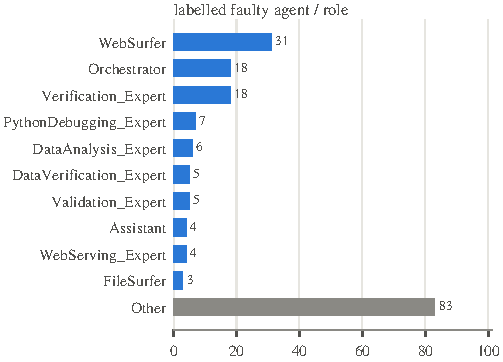
\includegraphics[width=\linewidth]{3_core/who_and_when/figures/agent.pdf}
\end{minipage}

\paragraph{Example trajectory} Hand-Crafted log \code{48.json} (AssistantBench; 5 steps, 2 agents, 12\,k characters). The WebSurfer issues a search, never reads a weather source, and the run ends with an unsupported answer.
% auto-generated by scripts/render_traj.py -- do not edit
\trajtask{Hand-Crafted/\allowbreak{}48.json}{Based on recent years (2020-2023),\allowbreak{} how likely am I to hit a rainy day (at least 0.5mm of precipitation) if I travel to Seattle during the first week of September?\allowbreak{} (provide the answer in percentage)}
\begin{trajstep}{0}{human}{agA}
Based on recent years (2020-2023),\allowbreak{} how likely am I to hit a rainy day (at least 0.5mm of precipitation) if I travel to Seattle during the first week of September?\allowbreak{} (provide the answer in percentage)
\end{trajstep}
\begin{trajstep}{1}{Orchestrator (thought)}{agB}
Initial plan:\allowbreak{}\par We are working to address the following user request:\allowbreak{}\par Based on recent years (2020-2023),\allowbreak{} how likely am I to hit a rainy day (at least 0.5mm of precipitation) if I travel to Seattle during the first week of September?\allowbreak{} (provide the answer in percentage)\par To answer this request we have assembled the following team:\allowbreak{}\par Assistant:\allowbreak{} A helpful and general-purpose AI assistant that has strong language skills,\allowbreak{} Python skills,\allowbreak{} and Linux command line skills.\newline ComputerTerminal:\allowbreak{} A computer terminal that performs no other action than running Python scripts (provided to it quoted in ```python code blocks),\allowbreak{} or sh shell scripts (provided to it q\newline [...] (2,\allowbreak{}122 chars omitted) [...]\newline /\allowbreak{}usr/\allowbreak{}local/\allowbreak{}lib/\allowbreak{}python3.11/\allowbreak{}site-packages/\allowbreak{}autogen\_magentic\_one/\allowbreak{}agents/\allowbreak{}orchestrator.py:\allowbreak{}216:\allowbreak{} UserWarning:\allowbreak{} Resolved model mismatch:\allowbreak{} gpt-4o-2024-08-06 !=\allowbreak{} gpt-4o-2024-05-13. Model mapping may be incorrect.\newline ledger\_response =\allowbreak{} await self.\_model\_client.create(
\end{trajstep}
\begin{trajstep}{2}{Orchestrator (thought)}{agB}
Updated Ledger:\allowbreak{}\newline \{\newline "is\_request\_satisfied":\allowbreak{} \{\newline "reason":\allowbreak{} "The request has not yet been satisfied as we still need to gather and process the historical weather data for Seattle for the first week of September from 2020 to 2023.",\allowbreak{}\newline "answer":\allowbreak{} false\newline \},\allowbreak{}\newline "is\_in\_loop":\allowbreak{} \{\newline "reason":\allowbreak{} "We are not in a loop as we have just defined the plan and steps to proceed.",\allowbreak{}\newline "answer":\allowbreak{} false\newline \},\allowbreak{}\newline "is\_progress\_being\_made":\allowbreak{} \{\newline "reason":\allowbreak{} "We have outlined a clear plan and have just begun by initiating the request to gather data.",\allowbreak{}\newline "answer":\allowbreak{} true\newline \},\allowbreak{}\newline "next\_speaker":\allowbreak{} \{\newline "reason":\allowbreak{} "WebSurfer needs to search for and gather the necessary hi\newline [...] (231 chars omitted) [...]\newline er from 2020 to 2023.",\allowbreak{}\newline "answer":\allowbreak{} "Please search for historical weather data for Seattle for the first week of September from 2020 to 2023 and find the number of rainy days (with at least 0.5mm of precipitation) during that period each year."\newline \}\newline \}
\end{trajstep}
\begin{trajstep}{3}{Orchestrator (-> WebSurfer)}{agC}
Please search for historical weather data for Seattle for the first week of September from 2020 to 2023 and find the number of rainy days (with at least 0.5mm of precipitation) during that period each year.
\end{trajstep}
\begin{faultystep}{4}{WebSurfer}{agD}
I typed 'Seattle historical weather data September 2020-2023' into '0 characters out of 2000'.\par Here is a screenshot of [Seattle historical weather data September 2020-2023 - Search](https:\allowbreak{}/\allowbreak{}/\allowbreak{}www.bing.com/\allowbreak{}search?\allowbreak{}q=\allowbreak{}Seattle+historical+weather+data+September+2020-2023\&form=\allowbreak{}QBLH\&sp=\allowbreak{}-1\&lq=\allowbreak{}0\&pq=\allowbreak{}\&sc=\allowbreak{}0-0\&qs=\allowbreak{}n\&sk=\allowbreak{}\&cvid=\allowbreak{}273959149E7F422CB8DC7E6C09666674\&ghsh=\allowbreak{}0\&ghacc=\allowbreak{}0\&ghpl=\allowbreak{}). The viewport shows 31\% of the webpage,\allowbreak{} and is positioned at the top of the page.\newline The following metadata was extracted from the webpage:\allowbreak{}\par \{\newline "meta\_tags":\allowbreak{} \{\newline "referrer":\allowbreak{} "origin-when-cross-origin",\allowbreak{}\newline "SystemEntropyOriginTrialToken":\allowbreak{} "A1L3tx5CzccqjN3lK6st/\allowbreak{}fXMwhf9EeokC\newline [...] (2,\allowbreak{}605 chars omitted) [...]\newline prompt and retry. To learn more about our content filtering policies please read our documentation:\allowbreak{} \textbackslash{}r\textbackslash{}nhttps:\allowbreak{}/\allowbreak{}/\allowbreak{}go.microsoft.com/\allowbreak{}fwlink/\allowbreak{}?\allowbreak{}linkid=\allowbreak{}2198766.",\allowbreak{} 'param':\allowbreak{} 'prompt',\allowbreak{} 'type':\allowbreak{} None\}\}\newline FINAL ANSWER:\allowbreak{} 20\newline SCENARIO.PY COMPLETE !\#!\#\newline RUN.SH COMPLETE !\#!\#
\end{faultystep}
\trajannotation{WebSurfer}{4}{—}{The agent didn't find enough information to answer the question but directly gave the answer.}{14.2}{I typed 'Seattle historical weather data September 2020-2023' into '0 characters out of 2000'.\par Here is a screenshot of [Seattle historical weather data September 2020-2023 - Search](http\newline [...] (7,\allowbreak{}160 chars omitted) [...]\newline ':\allowbreak{} None\}\}\newline FINAL ANSWER:\allowbreak{} 20\newline SCENARIO.PY COMPLETE !\#!\#\newline RUN.SH COMPLETE !\#!\#}{\textbf{subset}: Hand-Crafted; \textbf{question\_ID}: 2aa5dd83fbcd0dce9a3dd4592106e5b5edf738008d932e357d477bba80e59ccf; \textbf{level}: None; \textbf{is\_correct}: False; \textbf{source\_benchmark}: AssistantBench; \textbf{step\_indexing}: 0-based index into history (history[0] is the user question in Hand-Crafted)}


\paragraph{Notes} (i) Two regimes in one benchmark: short, synthetic-team logs (Alg.-Gen.) versus long Magentic-One logs (Hand-Crafted, 34 of 58 have $\ge$30 steps). (ii) Only agent \emph{outputs} are stored---no tool inputs, screenshots or environment state (the ``partial observation'' setting TraceElephant criticises). (iii) Label quirks: inconsistent agent-name casing (\code{WebSurfer}/\code{Websurfer}), AG values stored as quoted strings, field names differ between subsets (\code{groundtruth} vs \code{ground\_truth}), only 4 records carry a \code{mistake\_type}. (iv) Overlaps: the same logs are re-annotated by three experts in MP-Bench (177 of its 289 items); TraceElephant re-runs the same two MAS with full traces; Who\&When~Pro is the scaled-up, injected-failure successor.
